\documentclass[a4paper,11.5pt]{article}
\usepackage[latin1]{inputenc}
\usepackage[T1]{fontenc}
\usepackage[english]{babel}
\usepackage{graphicx}
\usepackage{amsmath}
\usepackage{amsfonts}
\usepackage{multirow}
\usepackage{booktabs}
\usepackage{bbold}
\usepackage{mathtools}
\usepackage{mathrsfs}
\usepackage{enumitem}
\usepackage{array}

\setlength{\parindent}{0pt}
\DeclarePairedDelimiter{\floor}{\lfloor}{\rfloor}
\DeclarePairedDelimiter{\ceil}{\lceil}{\rceil}

\newcommand{\vt}{\boldsymbol}

\title{Digital Communications - HW2}
\author{Jacopo Pegoraro, Edoardo Vanin}
\date{24/04/2018}

\begin{document}

\maketitle

\section*{Exercise 1}

We want to estimate the impulse response of an IIR real system affected by white noise and with different sampling period between the input and the output, putting ourselves at the receiver so knowing only the output of the system, the input and a bound on the order of the system (approximating the IIR with an FIR). In particular we call the input of the system $x(kT_x)$ with $T_x=1$, that undergoes upsampling of a factor 2 becoming $y(mT_y)$ with $T_y=\frac{T_x}{2}$ and is then filtered with an impulse response $h$ defined on $T_y$ that is what we want to estimate. To the output of the filter $z(mT_y)$ is added a white Gaussian noise $w(mT_y)$ with variance $\sigma_w^2=-8$ dB. We call the overall output after all these operations $r(mT_y)$. The difference equation of the filter is known at the transmitter and is, neglecting the dependance on $T_y$ for an easier notation:
\begin{equation} \label{eq:diff}
z(m)=-a_1z(m-1)-a_2z(m-2)+y(m)
\end{equation}
\noindent where $a_1=-0.9635$ and $a_2=0.4642$. 
To do the estimation we need to use as input a PN sequence and approximate the IIR filter with an FIR of order $N_h\le20$. However, we only know methods that can work if the input and the output of the filter are defined on the same sampling period, while in this case $h$ is defined on $T_y$. To solve the problem we exploit the polyphase representation of the system, dividing $h$ in $h^{(0)}$ and $h^{(1)}$ that act respectively only on the even and odd samples of the input (we are using the \emph{first noble identity} to transform the cascade of the upsampler and the filter in the separate filtering by $h^{(0)}$ and $h^{(1)}$ followed by a parallel to serial converter \cite{nevio<3}). Once the equivalent system is derived, we can perform separately the estimates of $h^{(0)}$ and $h^{(1)}$ that are now defined on the same sampling time as their input ($T_x$). Two different methods will be used on both the polyphase components: the correlation method and the least squares method (LS) \cite{nevio<3}. In the following sections we give a brief description of the structure of the PN sequences and of the two methods.

\subsection*{PN sequences}

PN sequences are deterministic and periodic binary sequences that, despite their non-random nature, present characteristics that make them suitable to simulate a white noise while being much more simple to generate \cite{nevio<3}. In this work we will use a type of PN sequences called Maximal Length sequences (ML) that can be obtained with recursive equations and the use of a shift register and the xor operator. ML sequences are defined giving their length $L$ that has to be an integer that precedes a power of 2 (here we will use sequences of length 7, 15, 31, 63, 127, 255). They can be generated starting with an arbitrary binary vector of length $r$ (where $r$ is the integer that satisfies $2^r -1=L$) and applying a difference equation that changes for every $L$ (we do not report her all the equations used and we refer to \cite{nevio<3}). The initial vector must not be the zero vector.
To estimate the channel we will use a ML sequence repeated 2 times to be able to eliminate the transient on the output when we need to, without computing the exact number of samples affected by transient behavior. The correlation and the mean of a ML sequence (using $-1$ and $1$ as binary values to eliminate biases) are:
$$
mean=\frac{1}{L}
$$
$$
r_{ML}=\begin{cases} 1 & \mbox{for  }  (n)_{modL} =0 \\
-\frac{1}{L} & \mbox{otherwise} \end{cases}
$$
\noindent that get closer to the ones of a white noise as $L$ increases. It's important to recall that to have good results in channel estimation using as input ML sequences we need to stick to the situation where $L$ is much bigger than $N$, otherwise the fact that mean and variance are not the same as a white noise will become more and more influent and affect the results.

\subsection*{Correlation method}

The correlation method is based on the schema represented in figure \ref{fig:systID}, but in our analysis we used $r(k)$ instead of $d(k)$ to be consistent with the notation.  

\begin{figure}[ht]
	\begin{center}    
		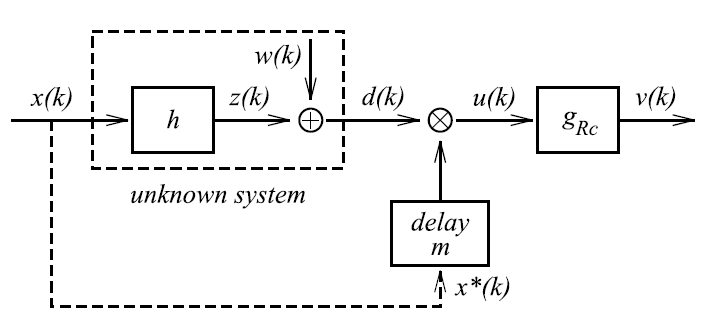
\includegraphics[width=10cm]{figs/systemID.png}
		\caption{Schema of the correlation method.}
		\label{fig:systID}
	\end{center}
\end{figure} 

\noindent The impulse response to be estimated is approximately equal to the correlation between the input sequence and the output of the unknown system (after the addition of the noise). The formula is:
\begin{equation} \label{eq:corr}
\hat{r}_{rx}(m)= \frac{1}{L} \sum_{k=L-1}^{2L-2}r(k)p^*(k-m)
\end{equation}
\noindent where we use the samples of $r(m)$ starting from $L-1$ to be sure we skip the transient. To adapt this procedure to our specific case we computed the output of the real system using its polyphase decomposition \footnote{In both the correlation method and the LS method the way we compute the target outputs is the same. Note that even if the given filter is IIR, a polyphase decomposition can be obtained anyway by exploiting the fact that Matlab approximates to 0 the taps of the impulse response after a certain value. The resulting outputs we obtain could have been equivalently derived by first computing the global output by upsampling $x(k)$, filtering with $h$ and in the end separating the even/odd sampler of $r(m)$. We chose the polyphase approach to avoid useless products by 0 in the filtering step.}. The result are the even/odd samples of the total output of the given system $r^{(0)}$ and $r^{(1)}$ that are the target outputs of the polyphase components, $h^{(0)}$ and $h^{(1)}$, to be used in \ref{eq:corr}. For each component then we carried out the computation of the correlation. The result is an estimate of the polyphase components from which we built the estimate $\hat{h}_{corr}$ of the complete impulse response by arranging the coefficients of the components as even and odd coefficients of $\hat{h}_{corr}$. As a measure of the error we make in estimating the coefficients we used the same functional as in the LS method (see the next section): $\mathcal{E}_{corr} = \sum_{k=L-1}^{2L-2}|r(k)-\hat{r}(k)|^2$, where $\hat{r}(k)$ is the output computed using the estimated impulse response. An estimate of the noise variance can be obtained with $\hat{\sigma}_{w,corr}^2=\frac{1}{L}\mathcal{E}_{corr} $.

\subsection*{LS method}

The LS method aims to minimize the functional $\mathcal{E} = \sum_{k=L-1}^{2L-2}|r(k)-\hat{r}(k)|^2$ where the expressions of the target output and the estimated output are:
\begin{equation}
r(k)=\vt{h}^T\vt{x}(k)+w(k)
\end{equation}
\begin{equation}
\hat{r}(k)=\hat{\vt{h}}^T\vt{x}(k)
\end{equation}
\noindent and we introduce the matrix $\vt{\Phi}$ and the vector $\vt{\theta}$:

\begin{equation}
\Phi (i,n)=\sum_{k=L-1}^{2L-2}x^*(k-i)x(k-n)
\end{equation}

\begin{equation}
\theta (n)=\sum_{k=L-1}^{2L-2}r(k)x^*(k-n)
\end{equation}
\noindent that have, respectively, dimensions $(L-1)\times(L-1)$ and $(L-1)\times 1$. To simplify the computation of the two quantities we introduce the data matrix $\boldsymbol{\mathcal{I}}$, defined as:

\begin{equation}
\vt{\mathcal{I}} =
\begin{bmatrix}
x(L-1)	& \cdots &	x(0) \\
\vdots	& \vdots & \vdots \\
x(2L-2)	& \cdots &	x(L-1)
\end{bmatrix}
\end{equation}
\noindent and the desired sample vector:
\begin{equation}
\vt{o}^T=[r(L-1) \ \ \ r(L-2) \ \ \  \dots \ \ \ r(2L-2)]
\end{equation}
\noindent from which we can obtain $\vt{\Phi}$ and $\vt{\theta}$ as  $\vt{\Phi}=\vt{\mathcal{I}}^H\vt{\mathcal{I}}$, $\vt{\theta}=\vt{\mathcal{I}}^H\vt{o}$. 
The solution of the LS estimate is given by $\hat{\vt{h}}_{ls}=\vt{\Phi}^{-1}\vt{\theta}$. 
As with the correlation method, here too the estimate is done separately for the 2 polyphase components by setting as target the output of the real system components $r^{(0)}$ and $r^{(1)}$. 

An estimate of the noise variance can be obtained with $\hat{\sigma}_{w,ls}^2=\frac{1}{L}\mathcal{E}_{ls} $ where $\mathcal{E}_{ls}$ is the mean squared error functional computed with the output obtained by filtering $x(k)$ with $\hat{h}_{ls}$.
\subsection*{Numerical Results}

To conduct a good estimation of the impulse response $h$ we need to carefully choose the 2 free parameters $L$, the length of the input PN sequence (that will be repeated 2 times), and $N$, the order of the filter that we know has to be assumed $\le20$. To do this we need to consider the resulting estimate of the noise variance derived from computing $\hat{h}$ with many different values of $N$ and $L$. The best choice will be the one that minimizes the variance (because that is related to minimizing the error, $\sigma_w^2\simeq \frac{\mathcal{E}_{min}}{L}$), without going below the performance bound of $-8$ dB, because in that case the estimate is affected by overfitting and is including the noise in the coefficients. In figure \ref{fig:L-N} we plotted the values of the variance of the noise for different $N$ and $L$, in dotted line for the correlation method and in solid line for the LS. We also added points to better understand where the estimate lies exactly with respect to the bound.
 \begin{figure}[ht]
	\begin{center}    
		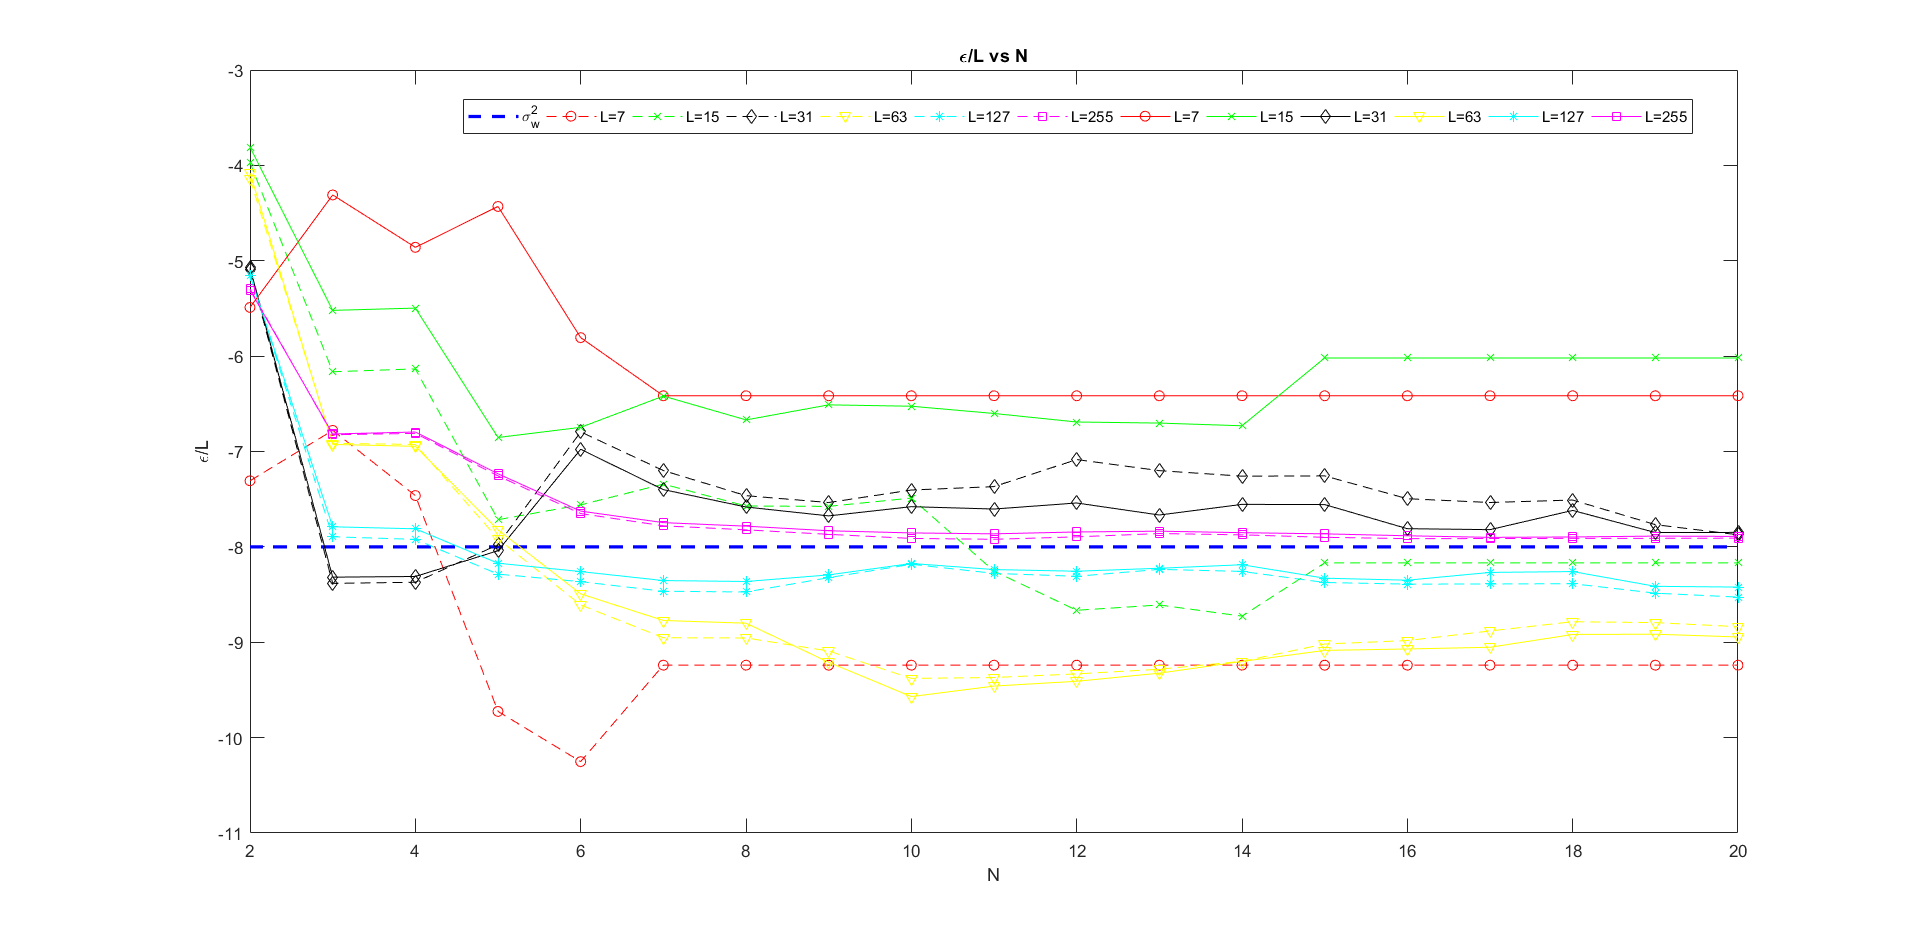
\includegraphics[width=\textwidth]{figs/L-N-choice.png}
		\caption{Plot of the estimated variance of the noise varying L and N.}
		\label{fig:L-N}
	\end{center}
\end{figure} 
\noindent We can see the for $L=7$ and $L=15$ the estimate does not show a stable behavior, while when $L$ increases we see a descending shape that approaches the bound or exceeds it. Good values of $L$ and $N$ can be $L=31$ and $N=5$ because in this point the estimated variance lies almost exactly on the bound. If instead we want to have a good estimate of more coefficients, $N=15$, $L=255$ could be another good choice. To keep the order of the filter as low as possible and to don't have to send a long sequence as input we decided for the first choice. In table 1 \ref{tab:coeff} we confront the estimated coefficients and the variance of the noise with their real values.

\begin{table}[htbp]
	\begin{center}
		\begin{tabular}{p{2.7cm}ccc}
			\toprule
			
			$nT_y$ & $h$ & $\hat{h}_{corr}$ & $\hat{h}_{ls}$\\
			\midrule
			0 & 1.0000  & 1.0054 & 0.9991  \\
			1 & 0.9635 & 0.9247 & 0.9613  \\
			2 & 0.4641 & 0.5002 & 0.5062 \\
			3 & -0.0001 & 0.0202 & 0.0255  \\
			4 & -0.2155 & -0.2549 & -0.2253\\
			\midrule
			%& \multicolumn{3}{c}{} \\
			& Real & Corr & LS \\
		    \cmidrule(lr){2-4}
		    $\sigma_w^2$ [dB] & -8 & -7.9776 & -8.0404  \\
			\bottomrule
		\end{tabular}
	\end{center}
	\label{tab:coeff}
	\caption{Estimated coefficients with the two methods for $N=5$ and $L=31$. Here are also reported the values of the estimated noise variance $\hat{\sigma}_w^2$.}
\end{table} 

\noindent We note that both methods perform well, and that the LS method is including a little noise into the estimate ($\frac{\mathcal{E}_{min}}{L}<\sigma_w^2$) but it's a very low value so we consider it not significant.

In figure \ref{fig:hest} we represent the analytical value of $h$ and the estimates.

\begin{figure}[ht]
	\begin{center}    
		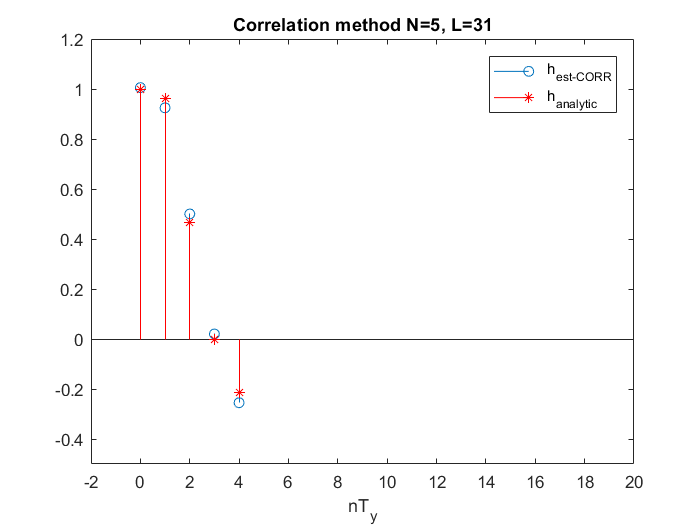
\includegraphics[width=6cm]{figs/corrN5L31.png}
		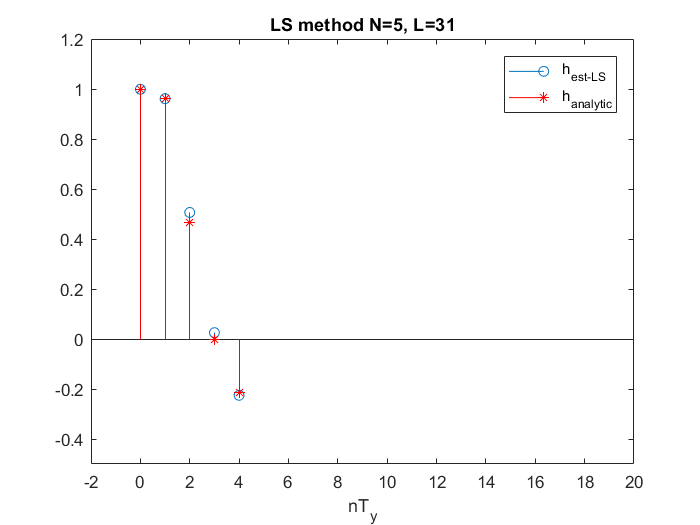
\includegraphics[width=6cm]{figs/lsN5L31.png}
		\caption{$h$ and $\hat{h}$ with the correlation and LS method for the final choice of the parameters L=31 and N=5 .}
		\label{fig:hest}
	\end{center}
\end{figure} 
 


\section*{Exercise 2}


\begin{figure}[ht]
	\begin{center}    
		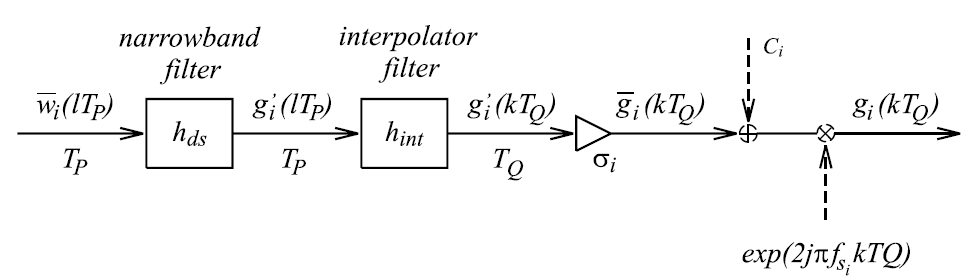
\includegraphics[width=10cm]{figs/ch-sim.png}
		\caption{Schema for the simulation of the channel impulse response.}
		\label{fig:ch-sim}
	\end{center}
\end{figure} 

We want to simulate a flat fading channel with impulse response given by just one tap $h_0(nT_c)$, and classical Doppler spectrum determined by $ f_d T_c = 40 \cdot 10^{-5} $. The Doppler spectrum model id defined as:
$$
\mathcal{D}(f)=\begin{cases}
                   \frac{1}{\pi f_d}\frac{1}{\sqrt{1-(f/f_d)^2}} & |f|\leq f_d \\
                   0                                             & \mbox{otherwise}   \\
                   
               \end{cases}
$$

 \noindent If the impulse response has a single tap this means we have only one component in the power delay profile, that is the first component made of a LOS real constant $C$ and a random part $\tilde{h}_1$ that we assume to be a complex Gaussian random process. We know that in this case the probability distribution function of $|\bar{h}_0|=|h_0/\sqrt{E[|h_0|^2]}|$ should be a Rice distribution, defined as \cite{nevio<3}:
\begin{equation}
p_{|\bar{h}_0|}(a)=2(1+K)ae^{-K-(1+K)a^2}I_0[2a\sqrt{K(1+K)}] \mathbb{1}(a)
\end{equation}
\noindent where $I_0$ is the modified Bessel function of the first type and order 0 and $K$ a parameter called Rice factor that is given $K_{dB}=2$ dB. The Rice factor is equal, in our case, to the ratio between the power of the direct component and the power of the reflected/scattered component: $K=\frac{C^2}{E[|\tilde{h}_0|^2]}$. If we assume we will normalize the power delay profile to 1, from the knowledge of $K$ we can derive $C=\sqrt{K/(K+1)}=0.783$. Then the power of the non direct component must be set equal to $M_d=1-C^2$ for normalization.

\subsection*{Simulation}


We start by assuming $T_c=1$. Following the schema in figure \ref{fig:ch-sim}, we generate a white noise with variance equal to 1 $\bar{w}_i(lT_p)$, defined of a sampling period $T_p$ bigger than $T_c$ such that $f_dT_p=0.1$ so $T_p=250$. This is necessary for the second step of the simulation, where we need to filter the white r.p. with an impulse response $h_{ds}$ given by the coefficients reported in \cite{ananas} to give it the shape of a classical Doppler spectrum (see figure \ref{fig:Ddoppler}). Indeed a convolution between $h_{ds}$ that has frequency content in the interval $[-f_d,f_d]$ and a process defined on $T_c$ would be practically non-feasible. It's important to recall that before filtering the coefficients must be normalized by the energy of the filter itself, to avoid unwanted modifications to the power of the r.p.. To go back to the original sampling time $T_c$ we used an interpolator filter for which we choose to use the spline interpolation method by a factor equal to $\frac{T_p}{T_c}=250$. 

\begin{figure}[ht]
	\begin{center}   
		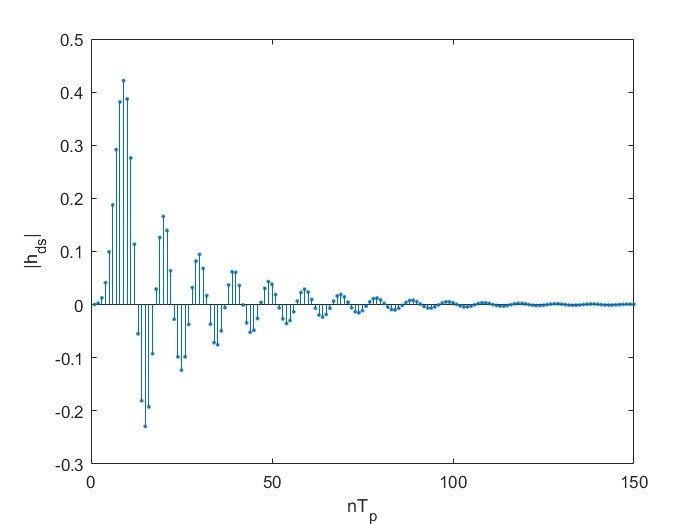
\includegraphics[width=6cm]{figs/hds.png} 
		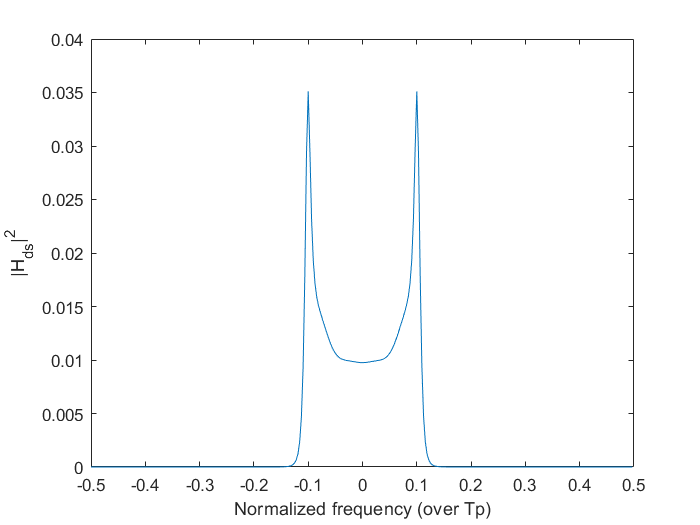
\includegraphics[width=6cm]{figs/dpspec.png}
		\caption{$h_{ds}$ and $|H_{ds}|^2$.}
		\label{fig:Ddoppler}
	\end{center}
\end{figure} 

\noindent After the interpolation we scaled the r.p. by a factor $\sqrt{Md}=0.622$, to give it the desired power level derived by the previous normalization. To complete the simulation we need to add the LOS component $C$ to each sample of the resulting r.p.. What we obtained is a simulation of $h_0(nT_q)$ that however contains a transient due to the Doppler spectrum filter that has to be dropped in order to have a stationary random process, and to do this we have 2 choices. Being the Doppler filter an IIR filter, we can compute the transient on the output as $N_{transient}\simeq 5N_{eq}\frac{T_p}{T_q}$ where $N_{eq}=\ceil{{\frac{1}{\ln(|p_{max}|)}}}=29$ is the equivalent time constant of the system (the number of samples needed to the strongest pole of the system to decade to $\frac{1}{e}$). We could also have made a more conservative choice by considering the truncation of the IIR impulse response made by Matlab and counting as transient its length, as we would do with an FIR filter. The results in the two cases are basically the same so we go for the first method. In figure \ref{fig:imp-resp} we show a plot of the resulting $|h_0(nT_c)|$ for 7500 samples once dropped the transient.

\begin{figure}[ht]
	\begin{center}    
		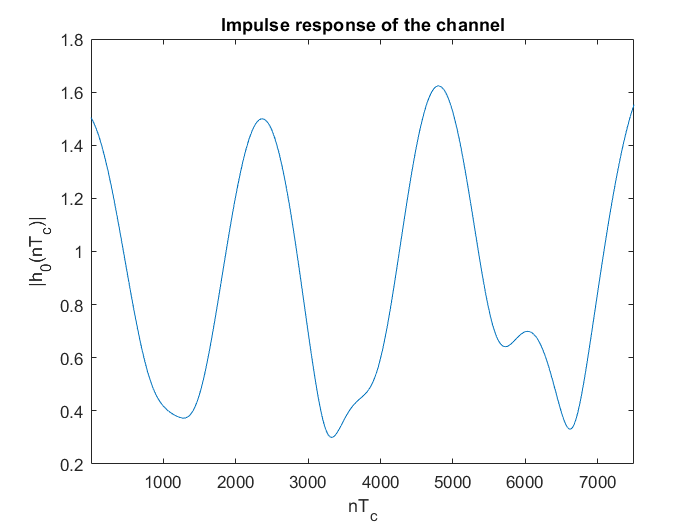
\includegraphics[width=10cm]{figs/imp-resp.png}
		\caption{Impulse response of the channel, plot for 7500 samples.}
		\label{fig:imp-resp}
	\end{center}
\end{figure}

\subsection*{Estimation of the pdf}

For the estimation of the pdf we used a vector of 80000 samples, removing an initial transient as described above. The resulting distribution should be a Rice distribution with parameter $K=1.5849$ in linear scale. In figure \ref{fig:histest} on the left we can see the results of an estimation with a histogram with 17 bins over the 80000 samples, plotted along the theoretical curve of the distribution. The estimate is enough accurate and follows quite well the asymptotic distribution. To give more quantitative results we also tried an estimate of the parameter $K$ using a Matlab function for the estimation of Rice distributions that uses a simple moment-matching approach \cite{rice}. The result on the same 80000 samples as in the histogram proves that the realization is very close to the theoretical result because the vale of $K$ obtained is $\hat{K}=1.5838$ that is almost equal to the real one as we can see again from figure \ref{fig:histest} on the right.

\begin{figure}[ht]
	\begin{center}    
		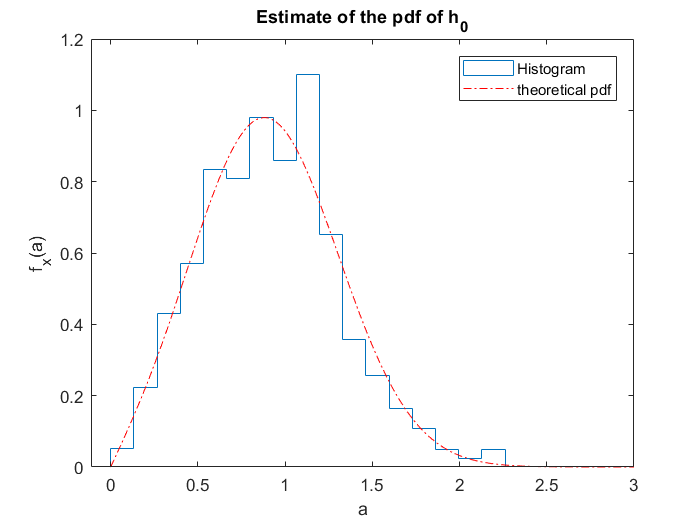
\includegraphics[width=6cm]{figs/hist-pdf.png}
		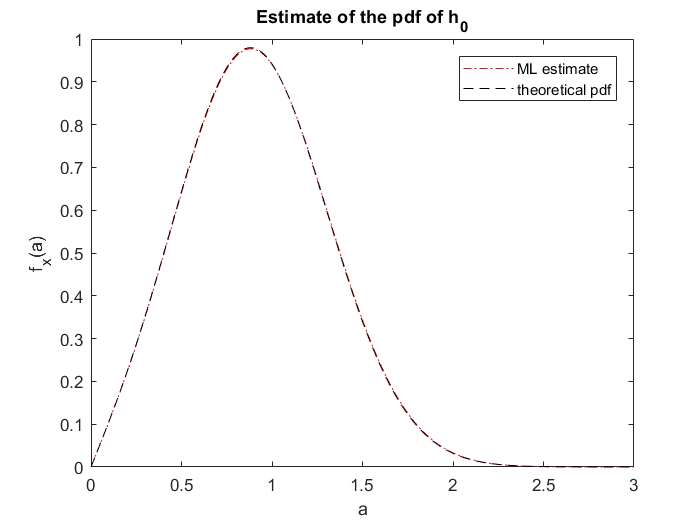
\includegraphics[width=6cm]{figs/ML-est.png}
		\caption{Estimate of the pdf of $|h_0|$ by an histogram (left) and with the use of an estimator for the parameter $K$.}
		\label{fig:histest}
	\end{center}
\end{figure}

\subsection*{Estimation of the PSD}

For the spectrum estimation we used the Welch periodogram method. This method consists in dividing the input sequence into subsequences of consecutive $D$ samples. Notice that two following subsequences, $h_0^{(s)}$ and $h_0^{(s+1)}$, overlap by $S$ samples. For our case we used $D =\frac{ \mbox{\# of samples}}{ 4}=20000$ and $S = \frac{D}{2}=10000$. \\


\begin{figure}[ht]
	\begin{center}    
		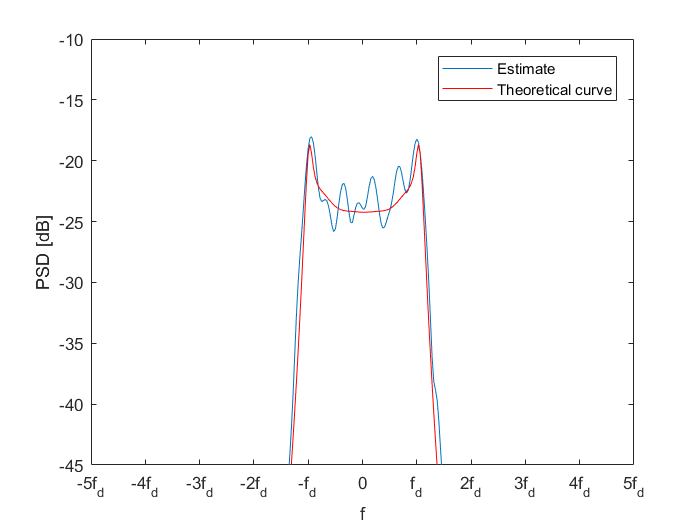
\includegraphics[width=10cm]{figs/PSD-est.png}
		\caption{Estimate of the PSD of $h_0$ with the Welch periodogram, $D=20000$ ad $S=10000$ with $80000$ samples.}
		\label{fig:PSD}
	\end{center}
\end{figure}
The number of subsequences is
\begin{equation}
N_s = \floor*{{\frac{K-D}{D-S}+1}}
\end{equation}

The Welch periodogram is computed as
\begin{equation}
\mathcal{P}_{WE}(f) = \frac{1}{N_s}\sum_{s=0}^{N_s-1}{\mathcal{P}}_{PER}^{(s)}(f)
\end{equation}

where ${\mathcal{P}}_{PER}^{(s)}(f)$ is the periodogram computed for $h_0^{(s)}$ using a window of length $D$. We chose an Hamming window. The result of the estimate can be seen in figure \ref{fig:PSD}, plotted along the theoretical curve obtained by considering a classical Doppler spectrum shape scaled by the power of $h_0$. Note that as we normalized the power of $h_0$ at the beginning, we don't need the normalization now to plot the results. The estimate seems to be pretty accurate, aside from some variance in the central region of the curve we are able to clearly see the side peaks of the classical Doppler spectrum.



\begin{thebibliography}{15}
	\bibitem{nevio<3}
	Nevio Benvenuto, Giovanni Cherubini,
	\textit{Algorithms for Communication Systems and their Applications}. 
	Wiley, 2002.
	
	\bibitem{ananas}
	A. Anastasopoulos and K. M. Chugg, 
	\textit{"An efficient method for simulation of frequency selective isotropic Rayleigh fading,"}
	1997 IEEE 47th Vehicular Technology Conference. Technology in Motion, Phoenix, AZ, 1997, pp. 2084-2088 vol.3.
	
	\bibitem{rice}
	Ged Ridgway,
	\textit{Rice/Rician distribution,}\\
	https://it.mathworks.com/matlabcentral/fileexchange/14237-rice-rician-distribution
	
	
\end{thebibliography}

\end{document}